%!TEX root = ../../../report.tex

\section{The jumping case} % (fold)
\label{sec:jumping_case}
Modeling the dynamics of walking gaits in a bipedal robot with 6 DOF has proved significantly complex and time consuming, even for the two-dimensional case.
However, it is necessary in order to calculate the most extreme torque and velocity values to apply to every joint during the motion and thus gauge the required motors for the application.
In order to ease the task, instead of calculating the motion equations for the walking or running cases, it was resolved to model the dynamics of the jump case.
This was decided under the assumption that a structure able to perform a static, vertical jump of a certain height $h$ and determined characteristics on one leg could be able to fulfill the power requirements necessary for running, both from an actuation and a structural point of view.
This assumption was built upon the findings introduced in \cite{jump-run1} and \cite{jump-run2}.

\subsubsection{Vertical jump dynamics} % (fold)
\label{ssub:static_jumping_dynamics}
As explained in section \ref{sec:dimensions}, the dimensions of the robot and its parameters have been conceived to imitate human characteristics and capabilities.
Therefore the jump analysis here will be carried out in resemblance of the human case, based on \cite{jump-dynamics1} and aiming at applying the results to a robot platform, as in \cite{jump-dynamics2}.
The jump case analyzed here can be described according to \cite{jump-dynamics1} as a static, squat jump over one foot with take-off and without counter-movement (SJ-NAS).
The whole jump cycle has been divided into two phases with different analysis: an impulse and an aerial period.

\begin{figure}[ht!]
    \centering
    \begin{subfigure}[b]{0.3\textwidth}
        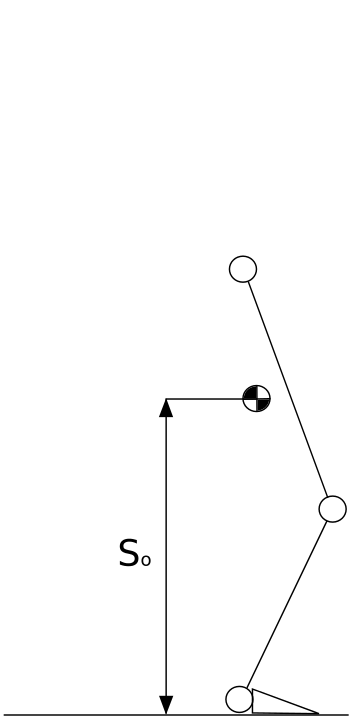
\includegraphics[width=\textwidth]{figures/launch_phase.png}
        \caption{Launch phase}
        \label{fig:launch_phase}
    \end{subfigure}
    \begin{subfigure}[b]{0.3\textwidth}
        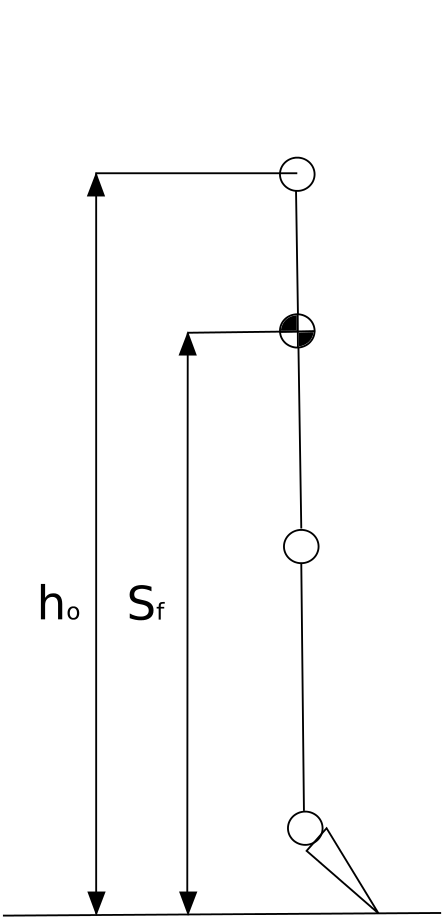
\includegraphics[width=\textwidth]{figures/takeoff_phase.png}
        \caption{Takeoff phase}
        \label{fig:takeoff_phase}
    \end{subfigure}
    \begin{subfigure}[b]{0.3\textwidth}
        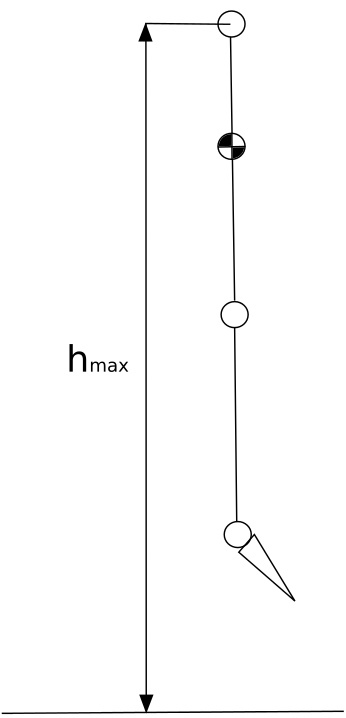
\includegraphics[width=\textwidth]{figures/flight_phase.png}
        \caption{Aerial phase}
        \label{fig:aerial_phase}
    \end{subfigure}
    \caption{Jump phases without fall and landing}
    \label{fig:jump_phases}
\end{figure}


\paragraph{The aerial phase}
The period from the take-off of the toes to the instant in which the maximum height $h_{max}$ has been reached, which can takes place between the instants represented in \ref{fig:takeoff_phase} and \ref{fig:aerial_phase}. 
The rest of the cycle, including fall and landing are not described here.
This phase is analyzed following the equations of a static projectile motion for the vertical launch case, expressed in \ref{eq:vertical_motion} and \ref{eq:vertical_energy}.

%\begin{equation}
%\label{eq:vertical_motion}	
%	h(t) = V_o t sin(\theta) - \cfrac{1}{2} g t^2 
%\end{equation}

\begin{equation}
\label{eq:vertical_energy}
	m g \Delta h = \cfrac{1}{2} m \Delta V^2
\end{equation}

The equation \ref{eq:vertical_energy} is an energy balance analysis for the flight phase, that can be rearranged as showed in \ref{eq:deltaV}

\begin{equation}
\label{eq:deltaV}
	\Delta V = \sqrt{2 g \Delta h}
\end{equation}

This equation can be used to input the desired displacement in the CoG of the robot during the free flight period and obtain the necessary velocity at take-off $V_{toff}$, which is the one the robot has to reach in the impulse phase.
This can be done since $V_{final} = 0$ and therefore $\Delta V = V_{toff}$.

\paragraph{The impulse phase}
From the initial position at the beginning of the jump, depicted in \ref{fig:launch_phase}, to the instant when the toes of the standing foot take off the ground and the ground reaction force ceases, shown in \ref{fig:takeoff_phase}.
The change in momentum in the robot, of mass $m$, caused by the application of a vertical force with the foot to the ground $F$ during a period $t$ is given by equation \ref{eq:impulse}, derived from the second law of motion of Newton.

\begin{equation}
\label{eq:impulse}
	F  t = m  \Delta V	
\end{equation} 

Substituting equation \ref{eq:deltaV} in \ref{eq:impulse}, the necessary impulse to reach the desired maximum height can be computed.
However, since the force applied to the mass and the application period cannot be decoupled from the result of the equation, an energy analysis has to be carried out together with a posterior optimization of the two values for the desired design of the robot.
Solving equation \ref{eq:impulse} for a small range of application time values and after computing \ref{eq:deltaV} with increasing values of $\Delta h$ in the range $[0.01,0.1]$ meters yields a reciprocal graph whose positive quadrant can be seen in Figure \ref{fig:f-t}

\begin{figure}[ht!]
	\centering
	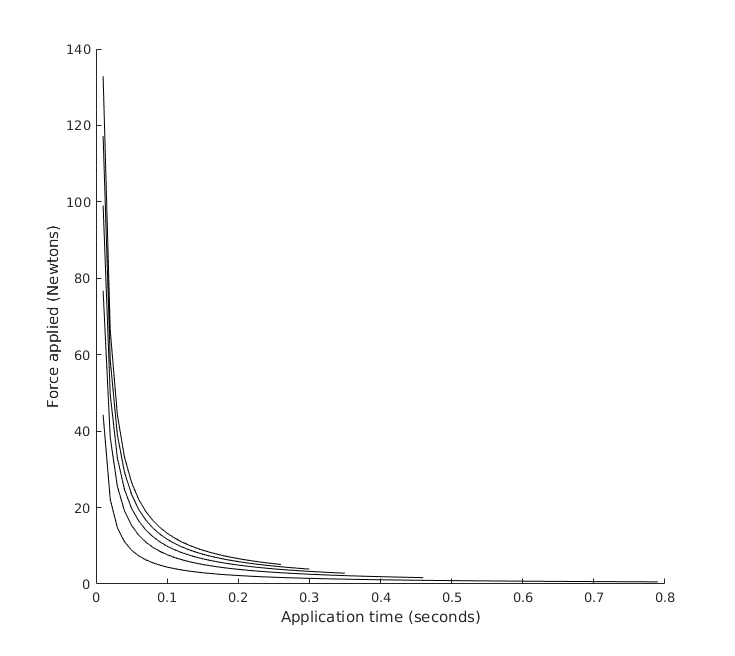
\includegraphics[width=0.8\textwidth]{figures/force-timePlot.png}
	\caption{Force-application time values for the same work magnitude}
	\label{fig:f-t}
\end{figure}

However, the obtained graphs do not propagate to an infinite value of application time, existing a boundary farther than which, the impulse will not produce enough variation in the momentum to launch the body.

\begin{equation}
\label{eq:work}
	W = \int_{t_{toff}}^{t_{f}} F(t)\,\mathrm{d}t = \cfrac{1}{2} m \Delta V^2 = F_{min} S
\end{equation}

Equation \ref{eq:work} describes how the work performed by the robot during the impulse phase can relate to the change in its kinetics energy. 
This equation, derived also from Newton's second law would only apply to rigid bodies without internal degrees of freedom, which is not the case.
However, it has been assumed that the displacement given by $S$ is the vertical translation of the CoM of the robot during the impulse and that it is small enough to be a valid assumption in order to use this procedure.
From Figure \ref{fig:jump_phases}, the displacement of the CoM during the impulse is given as $S=S_{f}-S_{o}$.
Knowing the value of $S$, the minimum necessary force can be obtained, and hence its corresponding application time on Figure \ref{fig:f-t} for a given $\Delta h$.
The displacement of the CoM, $S$ will depend on the initial configuration of the robot prior starting the impulse, and its final one.
Furthermore, for a given $\Delta h$, a range of possible values of the ground reaction Force $F$ can be computed within the limits established and a time can be obtained.
Thus, for a determined $\Delta h$ and $t$ values, a $F$ has to be applied by the foot again the ground.
In order to translate that force to joint effort, the dynamic model of the robot is required.

% subsubsection static_jumping_dynamics (end)

% section The_jumping_case (end)